\documentclass[12pt, letterpaper]{article}
\usepackage{graphicx}
\usepackage{siunitx}
\usepackage{fullpage}
\usepackage{setspace}
\usepackage{biblatex}
\usepackage{mathtools} 
\usepackage{appendix}
\usepackage[version=4]{mhchem}
\usepackage[export]{adjustbox}
\usepackage{pdflscape}
\usepackage{amsmath}
\graphicspath{{Images/}}
\addbibresource{sample.bib}
\doublespacing

\begin{document}

\begin{titlepage}
   \begin{center}
       \vspace*{1cm}

       \textbf{Modeling and Uncertainty Quantification of an MEA Absorption Column}
             
   \end{center}
\end{titlepage}

\newpage
  \tableofcontents
\newpage

\section{Introduction}

\paragraph{}
Carbon capture is recognized internationally as an indispensable key technology for mitigating climate change and protecting the human living environment \cite{Ma2022}. Carbon capture technologies have been developing since the 20th century but its modern conception for the means of reducing anthropogenic $CO_2$ emissions began in 1996 \cite{Ma2022}. There are many different types of carbon capture, but broadly there are three distinct technologies that exist: post-combustion, pre-combustion, and oxyfuel combustion. Post-combustion capture (PCC) is currently the most common and is primarily used and implemented in fossil-fuel power plants. The dominant technology used in PCC is absorption, or in other words, carbon scrubbing with amines, and is the only carbon capture technology currently used industrially \cite{CarbonCaptureTechs}. MEA (monoethanolamine) is the leading amine for this technology since it is the most understood chemically and has a high heat capacity since the solution contains mostly water. In order to better understand this technology and further its development, models are commonly built to simulate solvent-based PCC that occur at pilot plants around the world \cite{Oko2017}.

\paragraph{}
These models involve a full process system that includes many different unit models such as an absorption column, stripper column, mixers, heat exchangers, pumps, and condensers with the most significant being the absorption column.  This unit model contains the complex thermodynamics, kinetics, and transport physics that allow the $CO_2$ to be absorbed and great work has been done to better understand these three modeling components. The thermodynamic portion seems to be the most difficult to model since the amine mixture exhibits very non-ideal behavior since it contains strong associating interactions that can be difficult to track. Therefore, choosing and implementing a thermodynamic model is quite the task and is a cornerstone in absorption capture modeling. Models such as the e-NRTL (electrolyte non-random two-liquid) model have shown to be accurate \cite{Zhang2011} but recent development has shown that an advanced equation of state model like ePC-SAFT (electrolyte perturbed chain - statistical associating fluid theory) can lead to potentially even better accuracy \cite{Held2014}. Included in simulating this model are algorithms that approximate both the differential overall balance equations (mass and energy) of the system as well as relevant property models which help in determining the phase equilibrium of the system and thus the amount of $CO_2$ that can be captured. 

\paragraph{}
Just like the thermodynamic model, thermophysical and transport properties of species, mixture, and column play an important role in modeling carbon capture via absorption.  Thermophysical properties such as viscosity, density, and heat capacity, as well as transport properties such as inter-facial area or diffusivity, are examples of the relevant properties used and are approximated as a functional correlation dependent on temperature or concentration. Most of these functional correlations are obtained through regression analysis \cite{Morgan2017} and can be accurate but can also contain uncertainties and errors since it is difficult to fully characterize these complex and volatile properties with physics alone. In a recent development, an alternative approach such as utilizing physics-informed neural networks (PINNs) can potentially bridge the gap between what the functional correlations fail to capture and how these properties are truly characterized in real systems \cite{Morgan2017}. When the complexities of the thermodynamic model are combined with models that fail to accurately characterize each property, many uncertainties are found and can affect the overall accuracy of the model. Therefore, a key component of modeling carbon capture via absorption includes utilizing uncertainty quantification to characterize, trace, and manage all uncertainties of the model.

\paragraph{}
Uncertainty quantification (UQ) is the science of quantitative characterization and estimation of uncertainties in both computational and real-world applications. The uncertainties of carbon capture via absorption models are typically found in the thermodynamic model and property models given their complexity and volatility. Uncertainty quantification can be used to calibrate the parameters of these sub-models to better match the outputs of the model to the data gathered by pilot plants \cite{Morgan2018}. Since many simulations are needed, a surrogate model is used because it can very quickly run simulations of the model given that it accurately represents the model. With calibrated parameters and a more accurate process model from using ePC-SAFT and PINNs, an improved design of experiments can be made that aid in determining the next set of experiments to be run by a pilot plant. With these new experiments, updated results and data can be obtained and utilized to further calibrate the process model thus creating a cyclic process of better-run experiments and finely-tuned process models.

\paragraph{}
The goal of this work is to improve carbon capture via absorption modeling with various, novel contributions. The first contribution is to increase thermodynamic consistency by implementing the ePC-SAFT thermodynamic model in a full process model and comparing the results found with models that use the e-NRTL model. The next contribution is to improve the accuracy of relevant property models found in absorption modeling by utilizing physics-informed neural networks.  The final contribution is to make an upgraded design of experiments by utilizing an MCMC-calibrated surrogate model. This will be made with the improved process model simulation results that come from the first two contributions.  In order to accomplish these tasks, first a robust and accurate model of an absorption column using MEA as the amine will be built in the Python programming language which will further develop into a full process system model to aid in future research and development.

\newpage

\section{Background}

\paragraph{}
Mass adoption of carbon capture technologies by industries is lagging behind \cite{Ma2022}.  The main roadblock is the economic uncertainty of this technology so companies are apprehensive to invest in technologies that are untested and well-established \cite{Ma2022}. Modeling plays an important role in increasing this adoption of carbon capture technologies since it can provide a basis to better understand this technology and its economic margins.  Modeling can also provide development and testing without the consumption of expensive resources and time at pilot plants. Because of this, the Department of Energy (DOE) implemented a strong focus on the development of state-of-the-art process models and created the Carbon Capture Simulation for Industry Impact (CCSI2). CCSI2 develops, validates, and applies advanced computational techniques for technology simulation, optimization, uncertainty quantification (UQ), and process control \cite{NETLwebsite}. One of CCSI2's main goals is to develop  a rigorous, fast, and robust process model that can serve as a reference to test the performance of solvent-based PCC systems, with monoethanolamine (MEA) being used as a standard. These models can be simulated in traditional chemical engineering process simulation software but also in customized software built to fulfill the specific needs of research and development.

\paragraph{}
A significant component of developing a solvent-based PCC process model is designing the absorption column unit model that houses the complex thermodynamics, reaction kinetics, and transport that all play a vital role in the absorption of $CO_2$ into the aqueous amine solvent. Of these components, thermodynamics is the most significant since it predicts the phase-equilibrium of the system which provides the driving force of the absorption. This driving force can be seen as a measure of fugacity between the vapor and the liquid phases. To calculate fugacity, a thermodynamic model such as the e-NRTL (electrolyte Non-Random Two-Liquid) model can be used to represent the complex interactions that occur in the mixture. These models also provide the necessary equations that lead to fugacity and are specifically built and studied for these applications.

\paragraph{}
Similar to thermodynamic models, property models also play an important role in the absorption column. Fine-tuned property models are key in order to reaching the desired accuracy asked of these carbon capture process models. In general, these properties determine the mass transfer of the system, greatly influencing the flux between the phases for each species but most importantly $CO_2$. The properties include thermophysical properties such as viscosity, surface tension, density, diffusivity, and heat capacity as well as transport properties including interfacial area, hold-up, and others.  These properties are fitted to data and regressed to generate functional correlations dependent on either temperature, concentration, or both.  Depending on how the data was collected or the type of regression used uncertainties and errors are inevitable to be present. These properties often fail to match the characteristics that are often found and analyzed at pilot plants. 

\paragraph{}
Since these property models contain these uncertainties and errors, it is common to use uncertainty quantification as a tool for analysis and fine-tuning. Uncertainty quantification is a new and relevant priority for solvent-based PCC models yet there exists plenty of work and research already done showing the benefit that it can have \cite{Morgan2020}.  Uncertainty quantification can be used for analysis as well as calibration in solvent-based PCC models. A sensitivity analysis can be performed to determine how sensitive the quality of interest (QoI) is to an input parameter or a set of them. Fine-tuning of model parameters is also possible through MCMC (Markov Chain Monte Carlo) calibration and Bayesian regression. A surrogate model is often used in this application since it can quickly simulate the process model while testing multiple sets of parameters. These outputs are then matched up with data to determine the parameters that calibrate the process model closer to the pilot plant. 


\subsection{Research Motivation}

\subsubsection{Industry Adoption}
The difficulty of adopting carbon capture technologies in the industry is found in the economics. It is a large-scale process to implement and needs to achieve low energy consumption or lost cost when it is used for low-concentration emission sources (e.g., coal-fired and gas-fired power plants, steelworks, the cement and chemical industries, and waste incineration) \cite{Ma2022}. In addition to the high cost of investment in carbon capture facilities, there is still room for the optimization and improvement of the compression process and steam energy consumption; moreover, the very high solvent degradation rate requires the replenishment of solvents in large quantities during the operation of capture facilities, increasing the operating cost and the cost of capture.  Many of the above-mentioned performance issues are being solved.  For example, companies such as China Huaneng Group are exploring how to adjust the solvent makeup for each flue gas in order to  reduce degradation issues \cite{Ma2022}.  This shows the importance of modeling in reducing the cost of carbon capture and increasing the deployment of these technologies worldwide. 

\subsubsection{Modeling and CCSI2}

\paragraph{}
Modeling is a key component in advancing the technology of carbon capture and increasing its adoption. It can provide early drafts of processes as well as be utilized in fine-tuning an already existing carbon capture plant that is expected to adjust parameters and flue gas ratios. In a survey conducted by Huang, models have solved problems such as energy expansion planning, $CO_2$ network design problems, and $CO_2$ storage problems \cite{Huang2013}. Carbon capture models have also been used to test new and promising solvents that have been predicted to decrease cost and increase overall capture \cite{Oko2017}. Oko also explains how models are used to study the sensitivities of key process variables (e.g. capture level, solvent loading) at different operating conditions under steady state and dynamic scenarios and phenomena such as temperature bulge in the absorber \cite{Kvamsdal2008}. With this importance of modeling, the DOE created CCSI2 (Carbon Capture Simulation for Industry Impact) that focuses on developing a fundamental understanding of $CO_2$ capture technology.


\paragraph{}
The purpose of CCSI2 is to develop, validate, and apply advanced computational techniques for technology simulation, optimization, uncertainty quantification (UQ), and process control. Computational products are consolidated in the CCSI Toolset software for developing a rigorous understanding of $CO_2$ capture technologies that enable efficient Research and Development. CCSI2 develops a detailed multi-scale understanding of the most effective pathways to minimize the cost to capture CO2 \cite{NETLwebsite}.  The CCSI Toolset incorporates commercial and open-source software currently in use by the industry and is also developing new software tools as necessary to fill technology gaps identified during the execution of the project. Using the Toolset, CCSI2 collaborates with industrial, academic, and government partners to disseminate a rigorously quantified understanding of CO2 capture systems, manage risk and reduce the barriers to technology commercialization. \cite{NETLwebsite}. CCSI2 is currently developing a standard solvent-based CO2 capture system modeling framework with a fundamental multi-hierarchical characterization that will be used by the international CO2 capture industry to inform technology testing and development.


\subsubsection{Simulation Software}

\paragraph{}
 Traditional chemical process simulation software is often used to develop this process model.  A team at CCSI2 led by Morgan developed a very accurate and rigorous process model that was validated with steady-state data from the National Carbon Capture Center (NCCC) in Alabama \cite{Morgan2018}. Though the process model is rigorous and accurate, there still are problems that arose with its functionality. Unfortunately, traditional software is predominately made for the bulk, fine, specialty, and biochemical industries for the design, operation, and optimization of profitable manufacturing facilities.  When given a large, and random domain of input parameters and coefficients to simulate, the software runs into many convergence issues. When attempting to diagnose such issues, the lack of flexibility and customization offered by the software restricts the user to debug or revise the simulation.  This has cost many resources such as time and money for CCSI2 and alternative software has begun to be developed to circumvent these issues. 

\paragraph{}
A new process modeling software called IDAES (Innovative Development in Energy-Related Applied Science) is in development and is in collaboration with CCSI2. The aim of IDAES is to bring the most advanced modeling and optimization capabilities to solve the aforementioned challenges. The IDAES integrated platform utilizes the most advanced computational algorithms to enable the design and optimization of complex, interacting energy and process systems from individual plant components to the entire electrical grid. 

\begin{figure}[ht]
    \centering
    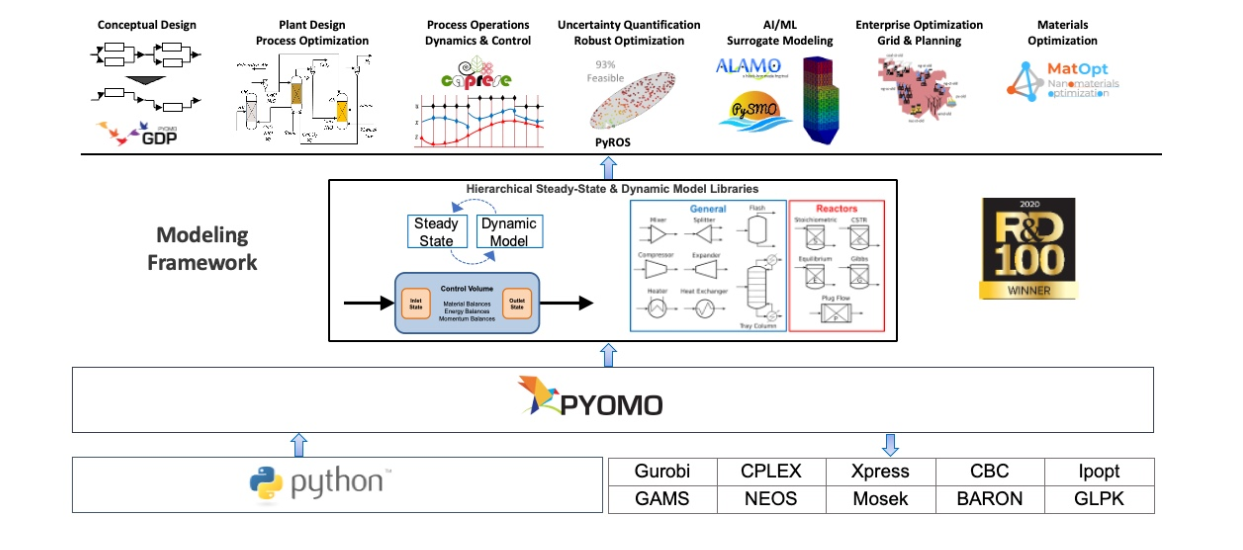
\includegraphics[width=16cm]{IDAES.png}
    \caption{IDAES Integrated Platform}
\end{figure}

\paragraph{}
Shown in Figure 1, The IDAES Integrated Platform consists of high-level capabilities (top row) that solve complex design and optimization problems with the Research and Development 100 award-winning core IDAES framework (middle row), which is implemented on top of state-of-the-art equation-oriented optimization solvers (bottom row). IDAES utilizes Pyomo, a Python-based, open-source optimization modeling language with a diverse set of optimization capabilities for formulating, solving, and analyzing optimization models. Though IDAES has a bright figure, it has still yet to have its first official release. The scope of the platform is very large and it takes much time for new additions and revisions to be made. IDAES is currently working on an Absorption Column unit model that is said to rival what is found in Aspen Plus, but it is currently under development and is not the main focus for the IDAES development team. Thus, another alternative was determined to be needed for bench-marking the uncertainty quantification of MEA-based carbon capture systems used by CCSI2.

\paragraph{}
Instead of using large-scale software, a custom process model from scratch was determined to be sufficient. This process model's focus would be on robustness, customization, and speed allowing it to be rigorously tested. A model built in Python was chosen due to the language's strength of customization and accessibility. In choosing this, speed was the biggest worry since Python sacrifices speed for ease of use and readability. Fortunately, this can be assisted with efficient algorithms run in faster languages and returned to Python. Developing a custom model in Python also provides the advantage of leveled complexity which either decreases or increases the overall depth of the model depending on the chosen constraints and assumptions. It also allows for the results of the simulation to be easily logged for future analysis. This can also provide a seamless integration between the modeling simulation and uncertainty quantification analysis.  In developing this process model, building the absorption column while integrating the thermodynamic framework provides the biggest challenge.

\subsection{Thermodynamic Framework}

\subsubsection{Absorption Column Fundamentals}
\paragraph{}
Understanding the fundamentals of an absorption column provides an important basis for developing a solvent-based PCC process model. For an MEA absorption column, there are many assumptions that can or cannot be made that drastically change the outlook of the model. 

\begin{figure}[ht]
    \centering
    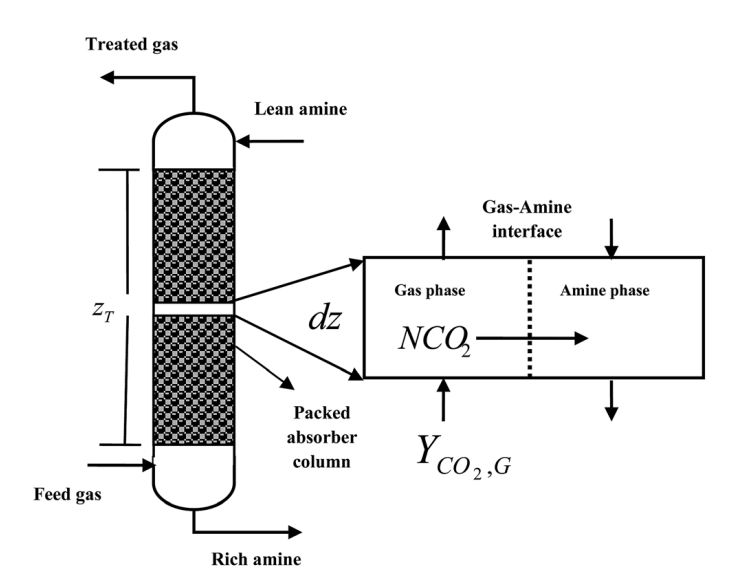
\includegraphics[width=12cm]{MEA_Absorption_Column}
    \caption{MEA Absorption Column}
\end{figure}

Figure 2 from \cite{Afkhamipour2017} above shows a diagram of an amine-based absorption column. It is a packed column with a variable height and diameter depending on the amount of liquid and vapor expected to be coming into the column. The column is packed with either random or structured packing that plays an important role in providing the surface area where the gas and liquid phases contact each other. A lean (which means it lacks the absorbed species being $CO_2$ in this case) amine solvent enters in from the top and an inlet flue gas coming from a post-combustion process enters in from the bottom. As the liquid falls and the vapor rises, the mixing happens on the packing at the phase interface. This causes both a reaction and absorption to occur which transfers the pollutant gas species of interest from the vapor to the liquid. The treated gas then comes out at the top and a rich (saturated with the absorbed pollutant) liquid amine solution comes out at the bottom.  Quantifying this transfer is key and is often modeled by the standard two-film theory (STFT) by Whitman \cite{Whitman1923} shown in Figure 3 \cite{Wang2018}.  

\begin{figure}[ht]
    \centering
    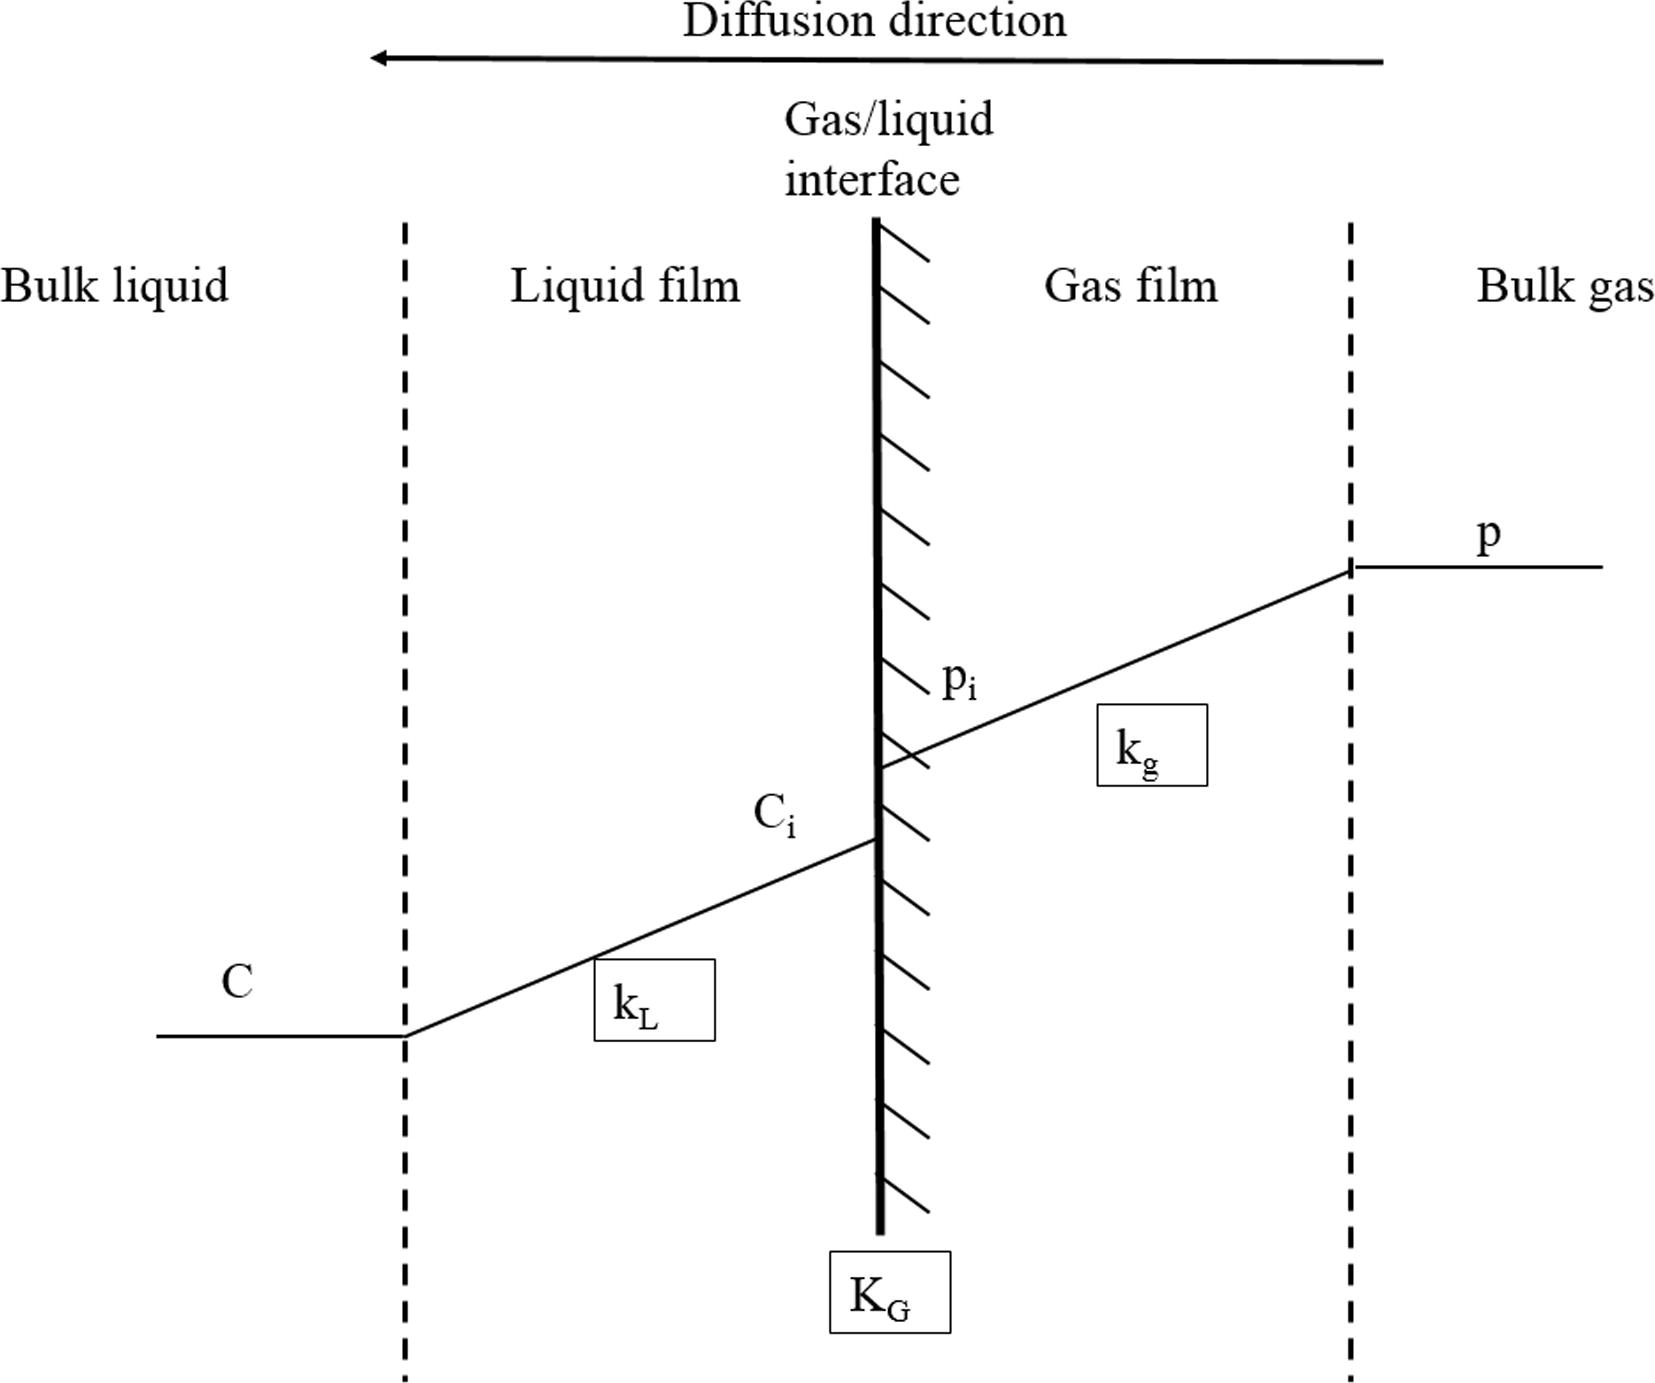
\includegraphics[width=12cm]{Two Film Theory.jpg}
    \caption{Standard Two Film Theory}
\end{figure}

Whitman showed that Fick's Law provides a linear concentration/pressure profile in the film, and the flux $N_i$ of species $i$ can be expressed as

\begin{equation}
N_i=k_l\left(C_{i,l}^{*}-C_{i,l}\right)=k_g\left(C_{i,v}-C_{i,v}^{*}\right)
\end{equation}

where $C_{i,j}^{*}$ is the interface concentration of species $i$ in phase $j$, $C_{i,j}$ is the bulk concentration of species {i} in phase {j}, and $k_j(\si{\meter\per\second})$ is the mass transfer coefficient for phase $j$. The vapor component can also be shown in terms of partial pressure. This equation shows the two distinct but important components of flux that cause the absorption:

\begin{equation}
\text{Flux} = \text{Mass Transfer Coefficient} \times \text{Driving Force}
\end{equation}

While the mass transfer coefficient component is largely composed of the physical properties of the mixture (viscosity, diffusivity, etc..), the driving force is thermodynamically driven by the concentration gradient, derived from the fugacity gradient.

\subsubsection{Thermodynamics of Solvent-Based PCC}
\paragraph{}
The thermodynamics of solvent-based PCC plays an important role in quantifying the driving force from Equation 2 $(C_{i,l}^{*}-C_{i,l})$. While the bulk concentration is easily quantified, the concentration at the interface presents a more difficult challenge to quantify. The main methods to quantify this interfacial concentration are with a vapor-liquid equilibrium (VLE) model and Henry's Law.  We start with the assumption that the vapor-liquid interface is at equilibrium which can be shown as

\begin{equation}
  \hat{f}_i^V=\hat{f}_i^L  
\end{equation}

Where the vapor fugacity is evaluated as
\begin{equation}
\hat{f}_i^V=y_i \varphi_i^V P
\end{equation}

and liquid fugacity is evaluated as
\begin{equation}
\hat{f}_i^L=x_i \varphi_i^L P \quad \text{or} \quad \gamma_i x_i f_i^o
\end{equation}

depending on the method used to evaluate the liquid fugacity.  Regardless of the method used, these fugacity values are used to determine the equilibrium coefficient for each species

\begin{equation}
K_i=\frac{y_i}{x_i}
\end{equation}

This is a powerful relationship since it can equate any mole fraction in one phase to the other. By gathering the equilibrium coefficient of each species and solving a system of equations, the concentration of the interface can be quantified.  As said before, the equilibrium coefficient is calculated through the fugacity of each species for each phase and the strategy will be different depending on the thermodynamic model used. 

\subsubsection{Relevant Thermodynamic Models}

\paragraph{}
The vapor-liquid equilibrium (VLE) of the $MEA-H_2O-CO_2$ system is notoriously difficult to model correctly and there is a copious amount of research done to better understand and quantify it \cite{Liu1999}. The complexity comes from the reaction that occurs when $CO_2$ is absorbed into the aqueous MEA solution generating multiple electrolyte species. These electrolytes bring many difficult-to-track interactions between all of the species in the solution, and these interactions can affect the behavior of the liquid at varying temperatures. 

\paragraph{}
There are two main methods of modeling thermodynamic systems; the residual method and the excess method. The residual method assumes a deviation from an ideal gas or fluid and that deviation can be calculated with an equation of state (EoS) that takes into account molecular interactions. The fugacity coefficient can then be calculated from this EoS by applying the necessary mixing rules and computing a compressibility factor. The excess method on the other hand assumes a deviation from an ideal mixture and activity coefficients are used to quantify this deviation as well as Henry's Law. The standard approach is to use the excess method (like an activity coefficient model) for the liquid phase, and the residual method (EoS) for the vapor phase but exceptions do occur. Once the methods are finalized, a thermodynamic model is chosen to provide the equations for each method. 

\paragraph{}
Typically for the $MEA-H_2O-CO_2$ system, an EoS like Peng-Robinson (PR) or Soave-Redlich-Kwong (SRK) is used for the vapor and the electrolyte non-random two-liquid (e-NRTL) activity coefficient model is used for the liquid. The thermodynamic model chosen for the liquid side tends to be more important compared to the vapor side due to the complex interactions in the amine-solution that can be difficult to quantify. The e-NRTL was originally developed by Austgen\cite{Austgen1991} and Zhang later shows the favorable comparison that the e-NRTL model results have to experimental data \cite{Zhang2011}. Given this proven accuracy, Morgan from CCSI2 adapted the model to his research and showed further validation with pilot plant data \cite{Morgan2017_Dis}. Even though the e-NRTL model produced these accurate results, CCSI2 still struggled with this model when rigorous testing was done to test a large domain of model parameters.  During these parameter runs, many convergence issues were found as well as thermodynamic inconsistencies given the unique parameter sets used.  This may have been due to the simulating software used but also the type of data that was used to regress the e-NRTL model parameters. This is still an ongoing issue for CCSI2 that has halted the analysis that can be done for these models. While the thermodynamic model is primarily responsible for quantifying the driving force of the flux, the physical properties of the species will specify the mass transfer coefficient which is the other puzzle piece in order to quantify the absorption of $CO_2$. 

\subsection{Physical Property Models in Solvent-Based PCC}

\paragraph{}
The predictive capability of rigorous process models is dependent on the accuracy of the underlying physical property models. These property models are generally responsible for the accuracy of the quantification of the transport phenomena occurring with the column. Quantifying the transport phenomena entails the computation of the mass transfer coefficient, interfacial area, as well as overall heat transfer coefficient. All of these depend on multiple different physical properties as well as thermophysical properties in order to be computed. The mass transfer coefficient as well as the interfacial area are the transport components in computing the molecular flux for absorption.

\paragraph{}
The mass transfer coefficients for a packed column are determined through the equations found by Billet \cite{Billet1999} where the liquid and vapor mass transfer coefficients are respectively

\begin{equation}
k_i^{\mathrm{l}}=C_{\mathrm{l}}\left(\frac{g \rho_{\mathrm{l}}}{\mu_{\mathrm{l}}}\right)^{0.167}\left(\frac{D_i^{\mathrm{l}}}{d_{\mathrm{h}}}\right)^{0.5}\left(\frac{u_{\mathrm{L}}}{a}\right)^{0.333}
\end{equation}

\begin{equation}
k_i^{\mathrm{v}}=D_i^{\mathrm{v}} C_{\mathrm{v}}\left(\frac{a}{d_{\mathrm{h}}}\right)^{0.5} S c_{\mathrm{v}}^{0.333}\left(\frac{u_{\mathrm{v}} \rho_{\mathrm{v}}}{a \mu_{\mathrm{v}}}\right)^{0.75} \sqrt{\frac{1}{\varepsilon-h_{\mathrm{L}}}}
\end{equation}

and the equation for the interfacial area also comes from Billet \cite{Billet1999} as

\begin{equation}
a_{\mathrm{h}}=1.5\left(\frac{a_{\mathrm{p}}}{d_{\mathrm{h}}}\right)^{-0.5}\left(\frac{\rho_{\mathrm{L}} u_{\mathrm{L}} d_{\mathrm{h}}}{\mu_{\mathrm{L}}}\right)^{-0.2}\left(\frac{\rho_{\mathrm{L}} u_{\mathrm{L}}^2 d_{\mathrm{h}}}{\sigma_{\mathrm{L}}}\right)^{0.75}\left(\frac{u_{\mathrm{L}}^2}{g d_{\mathrm{h}}}\right)^{-0.45}
\end{equation}

All of these equations contain important physical properties that greatly influence the absorption and accuracy of the model

\subsubsection{Relevant Properties Models}

\paragraph{}
The important properties found in these equations are viscosity ($\mu$), density ($\rho$),  diffusivity ($D$), and surface tension ($\sigma $). The other variables found in these equations are related to the packing material used. Each of these properties presents a unique challenge in quantifying accurately since each has unique characteristics related to this solution. 

\paragraph{}
If we consider viscosity, it can be difficult to capture the effects of high temperature and lower MEA weight percentage. In the works by Weiland \cite{Weiland1998} and Amundsen \cite{Amundsen2009}, certain parameters are neglected that can cause this difficulty and lower the accuracy of the model. Since it is important to test the model at these lower MEA weight percentages, it is important to include a model that includes these ranges. If the density is considered, it is common to derive the model without accounting for the presence of ionic species that is found in the $MEA-CO_2-H_2O$ system. For surface tension, a model from Jayarathna \cite{Jayarathna2013} was shown to accurately represent the experimental data, it has a major shortcoming in that it is only applicable to solutions with discrete values of MEA composition.  These are a few examples of the drawback that comes from relying only on empirical correlations to model these properties. 

\subsubsection{Inaccuracy of Empirical Correlations}

\paragraph{}
The property models that are implemented into process simulators use simple empirical correlations as well as contain simplifications even when based upon first principles. Though it is common for these property models to be accurate compared to the data they were generated from, they may fail to fully capture the phenomena if wider operating conditions are considered or if used in a unique and novel scenario that differs from the source of the data. Xiong \cite{Xiong2021} explains that the accuracy and applicability of the empirical law are strongly dependent on the quantity and quality of the data sample.  In practicality, this low-quality data set can have insufficient data, a skewed distribution, and low mergeable data due to collecting from different experiments with various processing parameters. A formula fitted by these low-quality data will show a low accuracy. Improving the quantity or quality of data samples under a consistent experimental condition is a feasible way to solve the problem, but it also means high experimental costs. This is a major roadblock for solvent-based PCC models and various techniques are researched and tested to circumvent these issues.  With this potential inaccuracy in property models, the uncertainty in these models is unavoidable, and quantifying this uncertainty is an important step to getting over this common roadblock.

\subsection{Uncertainty Quantification}

\paragraph{}
All models are exactly what they say they are, models. No model can perfectly mimic what it is trying to replicate but some can do quite well. In very complex models, it is a fair assumption to make that the model will always fall short in predicting the experimental data it is set to match. Given this assumption, models can work around this inevitable shortcoming and calibrate what is missing to better match the experiment. What is normally missing in a model is how the properties are measured and defined for a specific model. Some property models are set and defined for a specific set of conditions or measured in an isolated experiment away from a specific model. This discrepancy is the uncertainty that is found in these types of models and if they are calibrated to the unique conditions of the system, they can lead to better results. Each of these property models contains coefficients that were generated from an empirical correlation, normally through regression. If these coefficients can be tuned or calibrated to match the specific data that it is intended to match, the model can be better equipped to predict the $CO_2$ captured given a set of inputs. 

\subsubsection{Sensitivity Analysis}
Other than just calibrating the parameters, it is also significant to understand the parametric uncertainty for all of the physical property models considered. Parametric uncertainty of all property models is propagated simultaneously through the model in order to determine with parameters, and which properties, the process model is sensitive to. A Sobol sensitivity analysis can be used to determine the relative contribution of the uncertainty of each parameter to the uncertainty of the process variables is estimated. Sensitivity indices are calculated for the contributions of individual parameters $\left(S_i\right)$ and interactions among pairs $\left(S_{i j}\right)$ or groups $\left(S_{1,2, \ldots, k}\right)$ to the overall variability of the dependent variables. These terms satisfy the equation:

\begin{equation}
    \sum_{i=1}^k S_i+\sum_{1 \leq i<j \leq k} S_{i j}+\cdots+S_{1,2, \ldots, k}=1
\end{equation}

This equation then calls for $2^k - 1$ terms, so a surrogate can be used to produce the output variables which will greatly reduce the computational cost.

\subsubsection{Calibration and Design of Experiments}
\paragraph{}
The method in which these property sub-models are calibrated can be generally termed Bayesian inference. In the process of Bayesian inference, experimental data are used to update beliefs about the distribution of a set of parameters (in this context they are the coefficients of a property model). A prior distribution is an initial distribution based on one's previous beliefs about the parameters. This prior distribution comes from the deterministic property model. A posterior distribution is derived through Bayesian inference as an updated belief that takes the experimental data into account as evidence. 

\begin{figure}[ht]
    \centering
    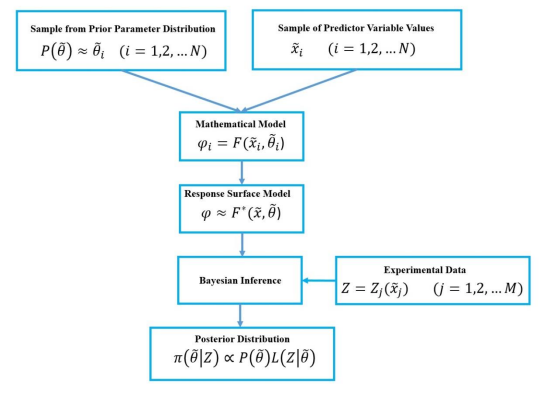
\includegraphics[width=16cm]{Bayesian Inference.png}
    \caption{Overview of UQ for Physical Property Models}
\end{figure}

Shown in Figure 3, is a diagram that outlines the process of developing a stochastic model for a property model. A response surface model is created to map the input values of the parameters and predictor variables to the output physical property value, which results in a reduction in the computational cost of Bayesian inference.  A surrogate response surface model is used in the application since 1000's or more simulations are needed to require an estimate of the posterior distributions. This posterior distribution is computed by the Markov Chain Monte Carlo (MCMC) method and is key to the uncertainty quantification done here.

\paragraph{}
Since uncertainty in physical property models is unavoidable, it is important that these uncertainties are quantified and considered when simulating the model.  Using Bayesian inference, the epistemic uncertainty can be considered and included in the process model so it behaves more like a realistic process.  Sensitivity analysis can also be used to better understand the contribution that each parameter and property has to the uncertainty found in the model.  This provided invaluable information to be better informed on the more relevant areas of the model and consider what future work should be made to improve and decrease that uncertainty.

\section{Work Plan}

\paragraph{}
The purpose of this work is to improve carbon capture via absorption modeling through various methods. The first is to develop a robust, yet rigorous process simulator with the ePC-SAFT thermodynamic model to predict the percentage of $CO_2$ captured. Next will be to integrate physics-informed neural networks (PINNs) to improve the relevant sub-models found in the process such as viscosity or surface tension.  The final method is to construct an improved surrogate model that can provide further analysis and assist in building a design of experiments to maximize the information content from experimental test runs at pilot plants.  

\begin{itemize}
  \item $\textbf{Task 1:}$ Develop a full $CO_2$ capture process simulator that includes the ePC-SAFT thermodynamic model
  \item $\textbf{Task 2:}$ Integrate physics-informed neural networks (PINNs) to improve relevant sub-models
  \item $\textbf{Task 3:}$ Develop an upgraded surrogate model to construct a design of experiments
\end{itemize}

\subsection{Task 1: Develop full process simulator with ePC-SAFT}

\paragraph{}
CCSI2 has a strong focus on the development of state-of-the-art process models and computational tools for
accelerating the development and commercialization of post-combustion carbon capture system technologies. As discussed before, the model built in traditional chemical processing software has its challenges so a new model was proposed to be built in Python to maximize robustness and speed. The foundations of this model have already been built and some of the progress made will be discussed here. This model was developed with multiple steps in mind. The first step was to build the absorption column unit model since it contains almost 90\% of the relevant information and physics involved in modeling carbon capture. This first step was then broken up into various stages that build on complexity as the model is developed. The first stage of the absorption column model was built with simplicity as the priority. This was completed rather quickly and laid the framework for building an absorption column model. The accuracy and validity of the model were not satisfactory so assumptions were removed and complexities were added until the model could be used for proper analysis. 

\paragraph{}
After some time, a new and updated version of the model was developed that could capture many more interactions that are involved in carbon capture. Unfortunately, each model run would take around 15 minutes to complete and the accuracy was still short of expectation. There was decent sensitivity for each input parameter, but due to the simulation time, the model was deemed almost unusable. For the next couple of months, every line of code and every equation was dissected and analyzed in order to reduce computational time.  The main culprit of the slow computation time was the shooting algorithm that was embedded with multiple non-linear solvers. Also, since there were many equations that contained non-linear logarithmic and exponential terms, any iteration with negative values caused the solver to diverge or break. This was a difficult problem to solve and both ingenuity and patience were required to gain any ground.  But after a couple of breakthroughs, the average simulation time came down to ten seconds, and a percent error for the solving algorithm averaged about $.005\% $. Some of these breakthroughs included fixing the shooting algorithm, maximizing code efficiency, and fine-tuning the non-linear solver parameters. This allowed for much better analysis and sampling and it is a highlight of this project. 

\paragraph{}
Given the speed of the run time, a Sobol sensitivity analysis could be performed to both test the model and determine the interactions between the input parameters. This sensitivity analysis had 384 runs to complete and the average percent error for the shooting accuracy was .040\%.  This percent error means that the shooting algorithm was able to converge on an answer that predicted a final $CO_2$ value matching the given value. Sobol indices display both first-order and second-order sensitivities. First-order sensitivities measure the fractional contribution of a single parameter to the output variance while second-order sensitivity indices are used to measure the fractional contribution of parameter interactions to the output variance. Both are shown below in Figure 4. It is easy to see that both $y_{CO_2}$ and $G$ take up most of the sensitivity fraction while the others have very little effect. This makes sense since both parameters influence the direct amount of $CO_2$ that is in the system, thus affecting the capture rate. The plot to the very right shows the second-order sensitivities and seems there are very few input interactions that are sensitive to the output.

\begin{figure}[ht]
    \centering
    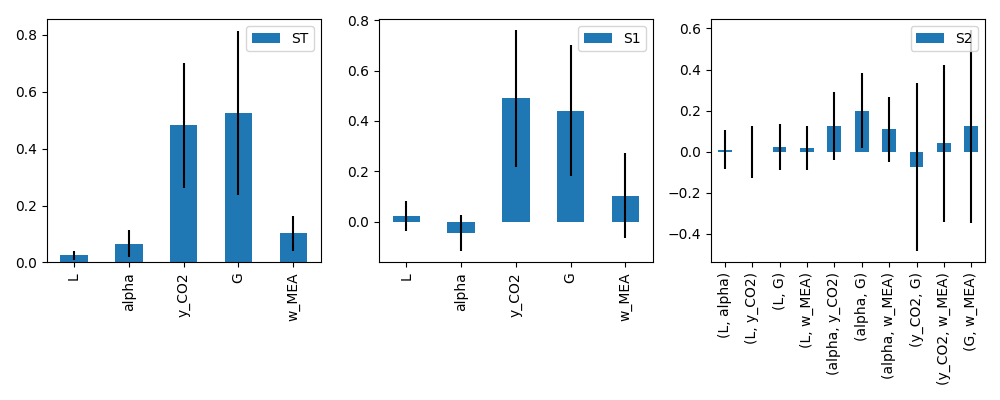
\includegraphics[width=16cm]{box.png}
    \caption{Box and Whisker Plot of Sensitivities}
\end{figure}

\paragraph{}
Although this model shows promising results and speed, there is plenty of room for improvement and further development needed. One of the main flaws of the model is the simplified thermodynamic framework that uses the Peng Robinson EoS to determine both liquid and vapor fugacity coefficients. This method is insufficient since it does not take into account the many interactions occurring in the liquid solvent. This leads to the next stage in the development of the absorption column model which involves updating the thermodynamic framework with a method that can account for those interactions. An obvious choice is to use the e-NRTL model for the liquid side since it has proven to match the literature data quite well \cite{Morgan2017}. The main equation for the e-NRTL model proposes that the excess Gibbs energy is given as a sum of these components:

\begin{equation}
    G^{e x}=G_{P D H}^{e x}+G_{\text {Born }}^{e x}+G_{L C}^{e x}
\end{equation}

The first two terms, the Pitzer-Debye-Hückel model and the Born equation are used to represent the contribution of the long-range ion-ion interactions. The third term, which includes the model parameters that may be adjusted to fit experimental data, represents the contribution of local interactions. 

\paragraph{}
Another potential model that has seen very little involvement in carbon capture simulations is the ePC-SAFT EoS originally developed by Cameretti \cite{Cameretti2005}. PC-SAFT (perturbed chain SAFT) is an equation of state that is based on statistical associating fluid theory (SAFT). Like other SAFT equations of state, it makes use of chain and association terms developed by Chapman, et al from perturbation theory. However, unlike earlier SAFT equations of state that used unbonded spherical particles as a reference fluid, it uses spherical particles in the context of hard chains as reference fluid for the dispersion term \cite{Wikipedia_2023}. The equation of state is organized into terms that account for different types of intermolecular interactions, including terms for the hard chain reference, dispersion, association, polar interactions, and ions. The equation is most often expressed in terms of the residual Helmholtz energy because all other thermodynamic properties can be easily found by taking the appropriate derivatives of the Helmholtz energy.
\begin{equation}
    a=a^{\mathrm{hc}}+a^{\text {disp }}+a^{\text {assoc }}+a^{\text {dipole }}+a^{\text {ion }}
\end{equation}

Here $a$ is the molar residual Helmholtz energy.

\paragraph{}
There is no research done that compares these two rigorous methods in carbon capture simulations. There are promising insights to be found with this comparison and both will be adopted in this model to perform these comparisons. After integrating these new thermodynamic frameworks, one of the final (but large steps) is to develop and integrate the remaining unit models for the full simulation. This includes models for a stripper, heat exchanger, pump, reboiler, condenser, and some others. Fortunately, these models are much simpler and more straightforward to integrate and develop compared to the absorption column. With these models developed and integrated, full system simulations can be implemented and analyzed to gain comprehensive knowledge of the system as a whole.  Although physics-based simulations can potentially predict an output that matches experimental data, often times there are many roadblocks and hurdles that physical models struggle to clearn alone. 

\subsection{Task 2: Integrate physics-informed neural networks (PINNs)}

\paragraph{}
Rather than developing elaborate computer codes or finding the hidden physics of a system, machine learning has emerged as a promising alternative. Unfortunately, there still exist many drawbacks when using machine learning by itself, such as the requirement of big data in order to train deep neural networks. Big data is not often available and is especially not available in applications such as carbon capture where experiments are costly. To circumvent this problem, large sets of data can be replaced with physical laws that can add constraints and patterns just like data can. Such physics-informed neural networks (PINNs) integrate (noisy) data and mathematical models, and implement them through neural networks or other kernel-based regression networks. Moreover, it may be possible to design specialized network architectures that automatically satisfy some of the physical invariants for better accuracy, faster training, and improved generalization \cite{Karniadakis2021}.  PINNs have a very high potential in many aspects of carbon capture modeling but a few are highlighted here that seem most relevant. 

\paragraph{}
The thermodynamic framework of the model seems to be the most uncertain and carries the most instability. As a promising alternative to thermodynamic approaches, PINNs can be employed to predict the equilibrium solubility of CO2 in a wide range of absorbents. These algorithms can effectively reflect the complexity of a system and the inherent relationship between the features and the solubility with high confidence and precision. In addition to the thermodynamic framework, other important thermodynamic properties of the system that affect the overall performance of the carbon capture process can be predicted using PINN methods. Among these properties, the density, viscosity, and surface tension of the system can be correlated to operational parameters, such as the temperature and CO2 partial pressure, as well as the absorbent properties \cite{Rahimi2021}.  There are a vast number of applications that PINNs can be utilized within carbon capture modeling that can both increase the accuracy of the model as well as help determine optimal operational conditions and develop a design of experiment for future test runs. 


\subsection{Task 3: Develop a surrogate model to construct a design of experiments}

\paragraph{}
The last aspect of this work will be to design a surrogate model for the development of a design of experiments methodology. This methodology will provide test runs throughout the input range of interest while selecting points that have relatively high uncertainty. As experimental data are collected according to the test plan, the distributions of some of the model parameters are updated through Bayesian inference. The test plan is then updated based on the new estimates of the process uncertainty. This process is demonstrated in Figure 5 below as a flowsheet.

\begin{figure}[ht]
    \centering
    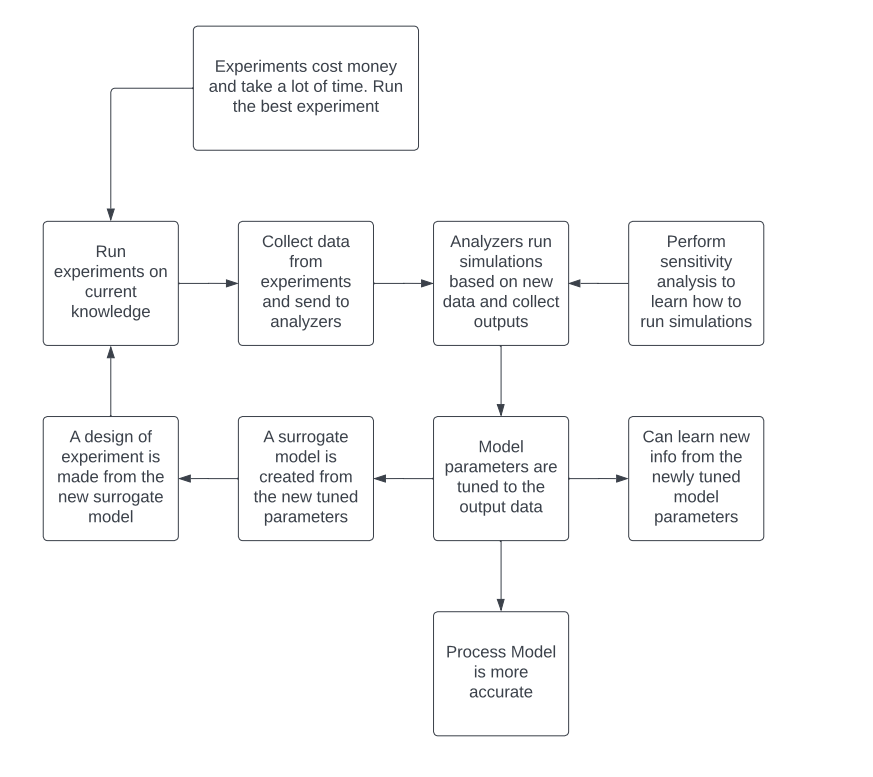
\includegraphics[width=14cm]{Flow Diagram.png}
    \caption{Flow Diagram of Design of Experiments Methodology}
\end{figure}

In the design of experiments methodology, the $\mathrm{CO}_2$ capture percentage of the absorber column is represented by a surrogate model, which may be denoted as:
\begin{equation}
    \hat{y}=\hat{y}\left(\tilde{x}, \tilde{\theta}_1, \tilde{\theta}_2\right)
\end{equation}

The set of independent variables, which is defined in Eq. 35, is denoted as $\tilde{x}$, and $\hat{y}$ refers to the response surface model prediction of the $\mathrm{CO}_2$ capture percentage. The model parameters are divided into two groups; $\tilde{\theta}_1$ refers to the set of parameters of fixed uncertainty and $\tilde{\theta}_2$ refers to the set of parameters for which the distributions are updated in light of the process data. There are two different groups of parameters since some parameters connected to physical properties have their uncertainty independent of plant hardware while others such as mass transfer and hydraulics models directly relate to plant hardware. 

\paragraph{}
To illustrate this concept, a surrogate model was created by simultaneously sampling from the input parameter distributions using MCMC. Figure 7 below shows a parity plot to demonstrate the quality of the response surface as a surrogate for the actual model. The response surface model developed using SEPIA (Simulation-Enabled Prediction, Inference, and Analysis) has been shown to be an adequate surrogate for the actual absorber process model, and the correlation between the two models has been calculated as $R^2$ $\approx$ .9978. In future work, this surrogate model will be created using both input variable distributions and 14+ parameter distributions from various property models and thermophysical models.

\begin{figure}[ht]
    \centering
    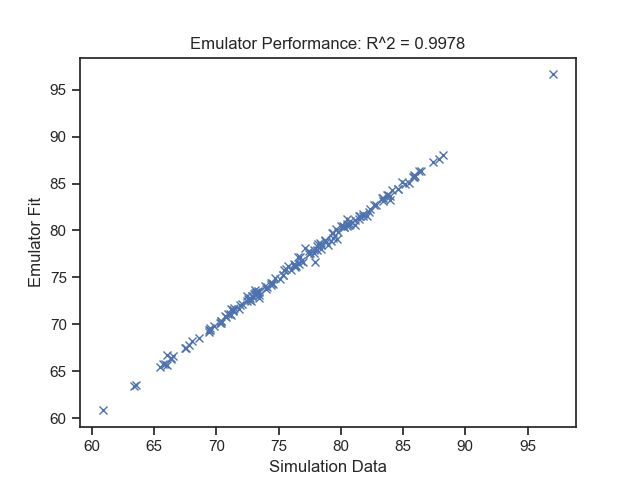
\includegraphics[width=14cm]{Emulator_Fit.png}
    \caption{Emulator Performance}
\end{figure}


\newpage

\begin{landscape}
\subsection{Project Timeline}

\begin{figure}[ht]
    \begin{center}
        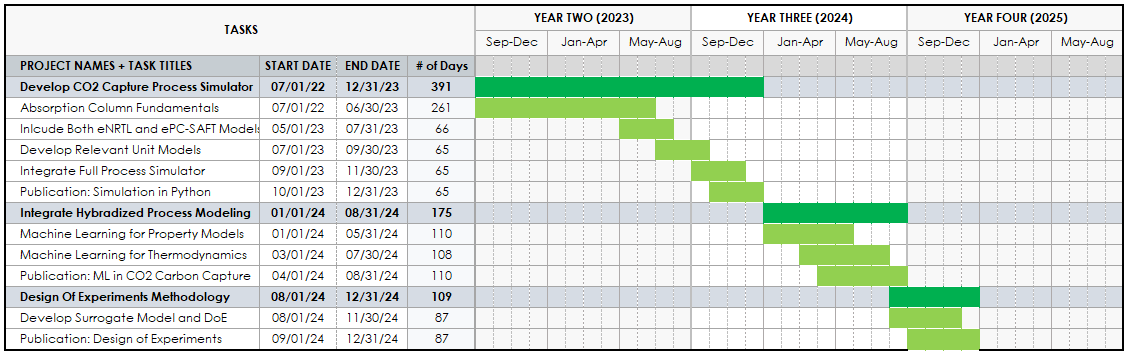
\includegraphics[width=22cm]{Project Timeline.png}
    \end{center}
    \caption{Project Timeline}
\end{figure}

\end{landscape}


\newpage

\printbibliography
\end{document}